%% =====================================================================
%%  Analisis Perbandingan Algoritma Welsh--Powell dan DSATUR untuk
%%  Penjadwalan Mata Kuliah Berbasis Pewarnaan Graf
%%
%%  IEEE conference template, A4, two columns, single author.
%%  Compile with:  latexmk -pdf main.tex
%% =====================================================================
\documentclass[conference,a4paper]{IEEEtran}

\usepackage[T1]{fontenc}
\usepackage[utf8]{inputenc}
\usepackage{amsmath,amssymb,amsfonts}
\usepackage{graphicx}
\usepackage{booktabs}
\usepackage{algorithm}
\usepackage{algpseudocode}
\usepackage{cite}
\usepackage{url}

% Shorthand for the two heuristics.
\newcommand{\WP}{\mathrm{WP}}
\newcommand{\DS}{\mathrm{DSATUR}}

\begin{document}

\title{Analisis Perbandingan Algoritma Welsh--Powell dan DSATUR untuk
Penjadwalan Mata Kuliah Berbasis Pewarnaan Graf}

%% ---------------------------------------------------------------------
%% METADATA PENULIS
%% ---------------------------------------------------------------------
\author{
\IEEEauthorblockN{Muhammad Akbar Yurizal Saputra}
\IEEEauthorblockA{%
Teknik Informatika\\
Fakultas Matematika dan IPA\\
Universitas Negeri Semarang\\
Semarang, Indonesia\\
akbaryurizal@students.unnes.ac.id}
}

\maketitle

\begin{abstract}
Penjadwalan mata kuliah dapat dipandang sebagai masalah pewarnaan graf: mata
kuliah menjadi simpul, dan dua mata kuliah yang diambil mahasiswa yang sama
dihubungkan oleh sisi karena tidak boleh menempati slot waktu yang sama.
Jumlah slot minimum sama dengan bilangan kromatik graf konflik, yang
komputasinya NP-\emph{hard}, sehingga praktiknya bergantung pada heuristik.
Penelitian ini membandingkan Welsh--Powell dan DSATUR \emph{greedy} secara
berpasangan pada 690 instans graf sintetis (600 graf acak Erd\H{o}s--R\'enyi
dengan $|V| \in \{20,40,60,80,100\}$, $p \in \{0.1,0.3,0.5,0.7\}$, 30 ulangan
per sel, dan 90 graf turunan simulasi pendaftaran), ditambah satu graf
pendaftaran nyata yang dianonimkan (156 mata kuliah, 975 mahasiswa) sebagai
studi kasus terpisah. Pasangan tersebut menghasilkan 690 perbandingan langsung
dan 1.380 eksekusi algoritma utama.
DSATUR menghasilkan rata-rata 11.10 warna dibandingkan 11.89 warna
Welsh--Powell, dengan reduksi rata-rata 7.17\% (uji peringkat bertanda Wilcoxon,
$p = 4.2\times10^{-66}$, $r = -0.95$), tetapi sekitar 3.09 kali lebih lambat.
Keunggulan DSATUR menyusut dari 11.14\% pada $p=0.1$ menjadi 5.49\% pada
$p=0.7$ dan praktis menghilang pada graf pendaftaran terstruktur (83 dari 90
instans seri). Pada 447 instans yang bilangan kromatiknya dibuktikan secara
eksak, celah rata-rata Welsh--Powell adalah 15.75\% dan DSATUR 7.06\%, dengan
DSATUR mencapai optimum pada 61.3\% instans. Pada graf nyata, $\chi(G)=13$
terbukti dan kedua heuristik mencapainya. Pilihan algoritma karena itu
bergantung pada tujuan: DSATUR untuk menekan jumlah slot pada graf acak yang
renggang dan besar, Welsh--Powell ketika waktu komputasi atau kesederhanaan
implementasi lebih penting.
\end{abstract}

\begin{IEEEkeywords}
pewarnaan graf, Welsh--Powell, DSATUR, penjadwalan mata kuliah, algoritma
heuristik, analisis komparatif
\end{IEEEkeywords}

\section{Pendahuluan}
Penjadwalan mata kuliah adalah persoalan operasional yang muncul setiap
semester. Inti persoalannya adalah menempatkan sejumlah mata kuliah ke dalam
slot waktu sedemikian rupa sehingga mata kuliah yang diambil oleh mahasiswa yang
sama tidak bertabrakan. Jika setiap mata kuliah menjadi simpul dan setiap
pasangan mata kuliah yang berbagi mahasiswa menjadi sisi, persoalan ini tepat
menjadi masalah pewarnaan simpul pada graf konflik: warna menyatakan slot waktu,
dan jumlah warna menyatakan jumlah slot yang dibutuhkan.

Pendekatan ini bukan hal baru. Hubungan antara penjadwalan dan pewarnaan graf
telah dirumuskan sejak karya Welsh dan Powell \cite{welsh1967upper}, yang
sekaligus memberikan batas atas bilangan kromatik dan menerapkannya pada
penjadwalan. Namun, meminimumkan jumlah warna berarti menentukan bilangan
kromatik $\chi(G)$, dan keputusan versi ini termasuk NP-\emph{hard}
\cite{karp1972reducibility,garey1979computers}. Untuk graf berukuran realistis,
jalan yang tersedia adalah heuristik: cepat, deterministik, dan selalu
menghasilkan pewarnaan sah, tetapi tanpa jaminan optimalitas.

Dua heuristik yang paling sering dirujuk adalah Welsh--Powell
\cite{welsh1967upper} dan DSATUR \cite{brelaz1979new}. Welsh--Powell mengurutkan
simpul menurut derajat menurun lalu mewarnai secara \emph{greedy}; DSATUR
memilih simpul berikutnya berdasarkan derajat saturasi, yaitu banyaknya warna
berbeda yang sudah dipakai tetangganya. Literatur sering menyatakan DSATUR
lebih baik, tetapi pernyataan itu umumnya berasal dari pengamatan pada kelas
graf tertentu atau dari eksperimen yang tidak dirancang berpasangan. Klaim
semacam itu perlu diuji ulang secara terkendali, terutama karena DSATUR
mengandung biaya komputasi tambahan yang jarang diukur secara adil.

Penelitian ini menjawab empat pertanyaan penelitian. \textbf{RQ1:} algoritma
mana yang menghasilkan warna lebih sedikit? \textbf{RQ2:} bagaimana kepadatan
graf memengaruhi jumlah warna kedua algoritma? \textbf{RQ3:} bagaimana ukuran
dan kepadatan graf memengaruhi waktu eksekusi terukur? \textbf{RQ4:} pada
kondisi graf mana masing-masing algoritma unggul atau seri?

Kontribusi yang dilaporkan bersifat empiris dan dapat direproduksi:
(i) implementasi kedua heuristik yang saling independen dan divalidasi silang;
(ii) rancangan eksperimen berpasangan pada 690 instans graf sintetis dengan
benih tetap, yang menghasilkan 690 perbandingan langsung dan 1.380 eksekusi
algoritma utama;
(iii) analisis statistik yang membedakan uji primer dari uji subkelompok yang
dikoreksi Holm; (iv) verifikasi bilangan kromatik eksak pada 447 instans
sehingga celah optimalitas dapat diukur, bukan diasumsikan; serta (v) satu studi
kasus pada graf pendaftaran nyata yang dianonimkan.

Sisa makalah disusun sebagai berikut. Bagian~\ref{sec:related} membahas
penelitian terkait dan landasan teori. Bagian~\ref{sec:model} merumuskan model
penjadwalan berbasis graf. Bagian~\ref{sec:algo} menjelaskan kedua algoritma
beserta analisis kompleksitasnya. Bagian~\ref{sec:method} memaparkan
metodologi eksperimen. Bagian~\ref{sec:results} menyajikan hasil dan
pembahasan, Bagian~\ref{sec:limits} keterbatasan, dan Bagian~\ref{sec:concl}
kesimpulan.

\section{Penelitian Terkait dan Landasan Teori}
\label{sec:related}

\subsection{Pewarnaan Graf}
Pewarnaan simpul yang sah memberikan warna berbeda kepada setiap pasangan
simpul bertetangga. Bilangan kromatik $\chi(G)$ adalah jumlah warna minimum
yang memungkinkan. Untuk setiap graf berlaku
\begin{equation}
\omega(G) \;\le\; \chi(G) \;\le\; \Delta(G)+1,
\label{eq:bounds}
\end{equation}
dengan $\omega(G)$ ukuran klik terbesar dan $\Delta(G)$ derajat maksimum.
Batas atas pada \eqref{eq:bounds} dijamin oleh pewarnaan \emph{greedy} dalam
urutan apa pun, sehingga kedua heuristik yang diteliti selalu menghasilkan
pewarnaan sah dengan paling banyak $\Delta(G)+1$ warna. Batas bawah $\omega(G)$
berguna untuk memverifikasi bahwa suatu hasil tidak dapat diperbaiki lagi pada
contoh-contoh kecil.

Welsh dan Powell \cite{welsh1967upper} memperkuat batas atas tersebut. Jika
$d_1 \ge d_2 \ge \dots \ge d_n$ adalah barisan derajat $G$, maka
\begin{equation}
\chi(G) \;\le\; 1 + \max_{1 \le i \le n} \min\left(d_i,\, i-1\right).
\label{eq:wpbound}
\end{equation}
Pertidaksamaan \eqref{eq:wpbound} menjelaskan mengapa pengurutan menurun
berdasarkan derajat masuk akal: simpul berderajat tinggi diberi warna lebih
awal, ketika masih banyak warna tersedia.

Br\'elaz \cite{brelaz1979new} mengusulkan DSATUR dengan gagasan berbeda:
alih-alih urutan statis, simpul dipilih secara adaptif berdasarkan derajat
saturasi, yaitu banyaknya warna berbeda pada tetangga yang sudah diwarnai,
sehingga simpul yang paling ``terjepit'' diproses lebih dahulu. Varian yang
diuji di sini adalah konstruksi \emph{greedy} DSATUR, bukan DSATUR eksak
berbasis \emph{branch-and-bound}. Survei Malaguti dan Toth
\cite{malaguti2010survey} serta buku Lewis \cite{lewis2021guide} menempatkan
keduanya sebagai heuristik konstruktif dasar, sedangkan de Werra
\cite{dewerra1990heuristics} dan Jensen dan Toft \cite{jensen1995graph}
membahas keluarga heuristik dan persoalan terbukanya. Keduanya juga dipakai di
luar penjadwalan, misalnya pada alokasi register \cite{chaitin1982register} dan
penjadwalan berskala besar \cite{leighton1979graph}.

\subsection{Penjadwalan Mata Kuliah}
de Werra \cite{dewerra1985introduction} memberikan pengantar formal penjadwalan
sebagai masalah pewarnaan dan pemartisian. Carter dkk.\
\cite{carter1996examination} merangkum strategi algoritmik untuk penjadwalan
ujian, sedangkan Burke
dan Petrovic \cite{burke2002recent} serta Burke dkk.\ \cite{burke2007graph}
menunjukkan bahwa heuristik berbasis graf tetap menjadi komponen penting di
dalam kerangka metaheuristik. Survei Babaei dkk.\ \cite{babaei2015survey}
menegaskan bahwa model graf konflik masih menjadi formulasi dasar.

Perbandingan empiris antarheuristik juga telah dilaporkan, misalnya oleh Healy
dan Ju \cite{healy2014experimental} pada graf acak renggang. Namun, studi
semacam itu jarang menyajikan perbandingan berpasangan yang mengendalikan
ukuran, kepadatan, dan struktur graf sekaligus, mengukur waktu dengan protokol
eksplisit, dan memverifikasi optimum. Celah itu yang diisi makalah ini.

\section{Model Penjadwalan Berbasis Graf}
\label{sec:model}

\subsection{Definisi}
Misalkan $V$ adalah himpunan mata kuliah dan $E$ himpunan pasangan mata kuliah
yang tidak boleh dijadwalkan bersamaan. Graf konflik didefinisikan sebagai
\begin{equation}
G=(V,E),
\label{eq:graph}
\end{equation}
dengan $|V|=n$ dan $|E|=m$. Untuk setiap mata kuliah $u \in V$, misalkan $S_u$
adalah himpunan mahasiswa yang mengambil $u$. Sisi muncul tepat ketika dua mata
kuliah berbagi paling sedikit satu mahasiswa:
\begin{equation}
E=\left\{\{u,v\}\subseteq V \;:\; u\neq v,\; S_u\cap S_v\neq\varnothing\right\}.
\label{eq:edges}
\end{equation}
Persamaan \eqref{eq:edges} adalah definisi operasional yang dipakai pada
Eksperimen~B: graf tidak diberikan secara langsung, melainkan diturunkan dari
tabel pendaftaran.

Pewarnaan $c: V \to \mathbb{N}_0$ dikatakan sah jika
\begin{equation}
c(u)\neq c(v), \qquad \forall \{u,v\}\in E .
\label{eq:valid}
\end{equation}
Jumlah warna yang dipakai adalah $k(c)=1+\max_{v\in V} c(v)$ untuk $V\neq
\varnothing$ dan $k=0$ untuk graf kosong. Tujuan optimisasi, dengan kendala
\eqref{eq:valid}, adalah
\begin{equation}
\begin{aligned}
\min_{c:\,V\to\mathbb{N}_0}\quad & k(c) \\
\text{subject to}\quad & c(u)\neq c(v),\quad \forall \{u,v\}\in E .
\end{aligned}
\label{eq:objective}
\end{equation}
Nilai optimum \eqref{eq:objective} adalah bilangan kromatik $\chi(G)$.

\subsection{Kepadatan dan Derajat Saturasi}
Kepadatan graf didefinisikan untuk $|V|\ge 2$ sebagai
\begin{equation}
d(G)=\frac{2\,|E|}{|V|\left(|V|-1\right)} \in [0,1].
\label{eq:density}
\end{equation}
Pada Eksperimen~A, $d(G)$ berbeda dari probabilitas pembangkitan $p$ karena
jumlah sisi yang terealisasi bersifat acak. Kedua besaran dilaporkan secara
terpisah dan tidak diperlakukan sebagai kuantitas yang identik.

Derajat saturasi yang menjadi dasar DSATUR didefinisikan sebagai
\begin{equation}
\operatorname{sat}(v)
=
\left|\left\{\,c(u) : u\in N(v),\ c(u)\ \text{sudah terdefinisi}\,\right\}\right|,
\label{eq:sat}
\end{equation}
dengan $N(v)$ himpunan tetangga $v$. Besaran \eqref{eq:sat} hanya menghitung
warna berbeda, bukan banyaknya tetangga yang sudah berwarna.

\subsection{Validasi dan Ukuran Kinerja}
Untuk memverifikasi bahwa suatu keluaran benar-benar sah, dihitung jumlah sisi
monokromatik
\begin{equation}
C(c)=\sum_{\{u,v\}\in E} \mathbf{1}\left[\,c(u)=c(v)\,\right],
\label{eq:conflicts}
\end{equation}
dan sebuah pewarnaan diterima hanya jika
\begin{equation}
C(c)=0 .
\label{eq:zeroconflict}
\end{equation}
Pemeriksaan \eqref{eq:zeroconflict} dijalankan pada setiap keluaran kedua
algoritma untuk seluruh 690 instans.

Reduksi jumlah warna DSATUR relatif terhadap Welsh--Powell didefinisikan
sebagai
\begin{equation}
R_k=\frac{k_{\WP}-k_{\DS}}{k_{\WP}}\times 100\%,
\label{eq:reduction}
\end{equation}
dengan $k_{\WP}$ dan $k_{\DS}$ berturut-turut jumlah warna kedua algoritma pada
graf yang sama. Nilai $R_k>0$ berarti DSATUR memakai warna lebih sedikit,
$R_k=0$ berarti seri, dan $R_k<0$ berarti Welsh--Powell lebih baik. Karena
penyebutnya $k_{\WP}$, nilai \eqref{eq:reduction} tidak terdefinisi untuk graf
kosong; graf kosong diuji terpisah dan tidak diikutkan dalam rata-rata.

\subsection{Asumsi dan Cakupan Model}
Meminimumkan jumlah warna setara dengan meminimumkan jumlah slot waktu hanya
jika setiap mata kuliah berdurasi sama, setiap slot berkapasitas tak terbatas,
dan tidak ada kendala lain. Model \eqref{eq:graph}--\eqref{eq:objective}
karena itu hanya menangkap konflik yang secara eksplisit terwakili sebagai
sisi. Ketersediaan dosen, kapasitas ruang, preferensi waktu, dan durasi kuliah
yang berbeda tidak dimodelkan.

Jumlah warna yang dihasilkan suatu heuristik $H$ merupakan batas atas yang
layak bagi bilangan kromatik, yaitu $\chi(G)\le k_H(G)$, sehingga $k_H(G)$
tidak selalu sama dengan bilangan kromatik $\chi(G)$. Optimalitas hanya
dinyatakan apabila $k_H(G)=\chi(G)$ dengan $\chi(G)$ dibuktikan secara eksak
dan independen. Suatu heuristik dapat optimal pada instans tertentu tanpa
jaminan umum, dan pembuktian $\chi(G)$ tidak menjamin seluruh heuristik
mencapainya. Keluaran penelitian ini karena itu adalah jumlah slot yang
dicapai heuristik menurut model tersebut, bukan jadwal universitas yang siap
pakai.

Sisi konflik dosen hanya dapat dibentuk jika data pendaftaran memuat penugasan
dosen untuk setiap mata kuliah. Dataset nyata yang dipakai pada Eksperimen~C
tidak memuat atribut tersebut, sehingga sisi dosen tidak dibentuk dan tidak ada
informasi dosen yang dikarang untuk melengkapinya. Dengan demikian model yang
dievaluasi tetap model konflik mahasiswa murni pada ketiga eksperimen, dan
perbandingan antareksperimen tetap setara.

\section{Algoritma Welsh--Powell dan DSATUR}
\label{sec:algo}

\subsection{Welsh--Powell}
Welsh--Powell mengurutkan simpul menurut derajat menurun dan memecah seri
berdasarkan pengenal simpul menaik, sehingga urutannya deterministik. Setiap
simpul kemudian menerima warna terkecil yang belum dipakai tetangganya.
Algoritma~\ref{alg:wp} menyajikan versi \emph{greedy} yang dipakai dalam
eksperimen.

\begin{algorithm}[!t]
\caption{Welsh--Powell (versi \emph{greedy})}
\label{alg:wp}
\begin{algorithmic}[1]
\Require graf $G=(V,E)$
\Ensure pemetaan warna $c:V\to\mathbb{N}_0$
\State $\sigma \gets$ urutan $V$ menurun menurut $\deg(v)$, seri menaik menurut $v$
\ForAll{$v\in\sigma$}
  \State $F\gets\{\,c(u) : u\in N(v),\ c(u)\ \text{terdefinisi}\,\}$
  \State $c(v)\gets\min\{\,j\in\mathbb{N}_0 : j\notin F\,\}$
\EndFor
\State \Return $c$
\end{algorithmic}
\end{algorithm}

Versi asli tahun 1967 membangun kelas warna satu per satu: ambil simpul belum
berwarna pertama dalam urutan, buka kelas baru, lalu sapu seluruh simpul belum
berwarna dan masukkan setiap simpul yang tidak bertetangga dengan anggota kelas
tersebut. Kedua formulasi ekuivalen: sebuah simpul selalu menerima indeks kelas
terkecil yang tidak memuat tetangganya, yang persis sama dengan warna terkecil
yang belum dipakai tetangganya. Kesetaraan ini diverifikasi secara eksekusi,
sehingga versi \emph{greedy} yang berbiaya lebih rendah dapat dipakai tanpa
mengubah hasil.

\emph{Kompleksitas.} Pengurutan memerlukan $O(n\log n)$. Pewarnaan memeriksa
setiap sisi satu kali dari sisi simpul yang sedang diwarnai, sehingga total
$O(n+m)$ dengan topeng bit untuk himpunan warna terlarang. Ruang yang
dibutuhkan $O(n+m)$.

\subsection{DSATUR}
DSATUR memilih simpul berikutnya secara adaptif. Aturan pemilihan yang dipakai
di sini, dan diterapkan secara konsisten, adalah: derajat saturasi
\eqref{eq:sat} terbesar; jika seri, derajat $\deg(v)$ terbesar; jika masih
seri, pengenal simpul terkecil. Setelah pemilihan, simpul menerima warna
terkecil yang belum dipakai tetangganya, lalu derajat saturasi para tetangganya
diperbarui. Algoritma~\ref{alg:dsatur} merangkum prosedurnya.

\begin{algorithm}[!t]
\caption{DSATUR \emph{greedy}}
\label{alg:dsatur}
\begin{algorithmic}[1]
\Require graf $G=(V,E)$
\Ensure pemetaan warna $c:V\to\mathbb{N}_0$
\State $c(v)\gets\text{belum berwarna}$ untuk semua $v\in V$
\While{ada simpul belum berwarna}
  \State pilih $v$ belum berwarna dengan $\operatorname{sat}(v)$ maksimum;
         seri: $\deg(v)$ maksimum; seri: $v$ minimum
  \State $c(v)\gets\min\{\,j\in\mathbb{N}_0 : j\notin\{c(u):u\in N(v)\}\,\}$
  \ForAll{$u\in N(v)$ yang belum berwarna}
    \State perbarui $\operatorname{sat}(u)$ menurut \eqref{eq:sat}
  \EndFor
\EndWhile
\State \Return $c$
\end{algorithmic}
\end{algorithm}

\emph{Kompleksitas.} Implementasi yang diuji menggunakan \emph{heap} biner
dengan pembatalan malas. Setiap simpul diwarnai tepat sekali, dan setiap
pewarnaan memeriksa seluruh tetangganya, sehingga total pemeriksaan $O(m)$.
Setiap kenaikan derajat saturasi mendorong satu entri ke \emph{heap} dengan
biaya $O(\log n)$, dan jumlah kenaikan dibatasi $\sum_v \deg(v)=2m$. Karena itu
waktu totalnya $O\!\left((n+m)\log n\right)$ dengan ruang $O(n+m)$.

Sebagai pembanding, implementasi acuan DSATUR yang memindai seluruh simpul
belum berwarna pada setiap langkah berjalan dalam $O(n^2+m)$. Kedua
implementasi diuji dan diwajibkan menghasilkan urutan pemilihan serta pewarnaan
yang identik, sehingga optimisasi struktur data tidak mengubah perilaku
algoritma.

\subsection{Catatan tentang Optimalitas}
Kedua algoritma merupakan heuristik konstruktif yang tidak memiliki jaminan
optimalitas secara umum. Meskipun demikian, optimalitas dapat dibuktikan pada
instans tertentu apabila jumlah warna yang dihasilkan sama dengan bilangan
kromatik $\chi(G)$ yang telah diverifikasi secara eksak. Pada graf lengkap
$K_n$ keduanya memang menghasilkan $n$
warna karena terpaksa, dan pada graf tanpa sisi keduanya menghasilkan satu
warna; kedua kasus itu dipakai sebagai uji kebenaran, bukan sebagai bukti
kinerja umum.

\subsection{Verifikasi Eksak dan Celah Optimalitas}
Perbandingan jumlah warna antara dua heuristik tidak dengan sendirinya
menunjukkan seberapa jauh keduanya dari optimum. Untuk mengukurnya, bilangan
kromatik dihitung secara eksak pada subhimpunan instans yang cukup kecil,
menggunakan pencarian \emph{branch-and-bound} berurut DSATUR. Pencarian memakai
batas atas berupa minimum dari solusi \emph{greedy} Welsh--Powell dan DSATUR,
serta batas bawah dari klik yang ditemukan secara \emph{greedy}; setiap langkah
memilih simpul belum berwarna dengan
derajat saturasi terbesar dan mencoba warna $0,\dots,\min(u,b-1)$, dengan $u$
banyak warna yang sudah terpakai dan $b$ solusi terbaik saat ini. Pencarian
dihentikan setelah batas waktu atau batas simpul, dan hasil yang tidak selesai
dilaporkan sebagai ``tidak terbukti'', bukan sebagai optimum.

Untuk instans yang $\chi(G)$-nya terbukti, celah optimalitas heuristik $H$
didefinisikan sebagai
\begin{equation}
G_H=\frac{k_H-\chi(G)}{\chi(G)}\times 100\%,
\label{eq:gap}
\end{equation}
dengan $k_H$ jumlah warna yang dipakai $H$. Nilai $G_H=0$ berarti heuristik
mencapai bilangan kromatik, sedangkan $G_H>0$ mengukur pemborosan relatif
terhadap optimum.

Untuk instans yang pencarian eksaknya tidak selesai, tidak ada celah yang dapat
dihitung. Yang dilaporkan adalah batas yang sah,
\begin{equation}
\omega(G)\;\le\;\chi(G)\;\le\;k^{*}(G),
\label{eq:gapbounds}
\end{equation}
dengan $k^{*}(G)=\min\{k_{\WP},\,k_{\DS}\}$, sehingga celah $H$ terkurung dalam
\begin{equation}
\begin{aligned}
\frac{k_H-k^{*}(G)}{k^{*}(G)}\times100\%
\;\le\;&G_H\\
\;\le\;&\frac{k_H-\omega(G)}{\omega(G)}\times100\% .
\end{aligned}
\label{eq:gapinterval}
\end{equation}
Pertidaksamaan \eqref{eq:gapinterval} adalah pernyataan tentang batas, bukan
hasil eksak, dan tidak pernah dilaporkan sebagai celah terukur.

Kebenaran pencarian eksak diverifikasi terhadap 120 graf acak kecil
($|V|\le 8$) yang bilangan kromatiknya dihitung dengan pencarian menyeluruh,
serta terhadap keluarga graf yang bilangan kromatiknya diketahui: $K_n$, siklus
ganjil dan genap, graf Petersen, graf Gr\"otzsch, graf bipartit lengkap,
hiperkubus, dan graf kisi. Seluruh 120 kasus acak dan seluruh keluarga uji
cocok.

\section{Metodologi Eksperimen}
\label{sec:method}

\subsection{Eksperimen A: Graf Acak}
Graf dibangkitkan dengan model Erd\H{o}s--R\'enyi $G(n,p)$
\cite{erdos1960evolution}. Untuk setiap pasangan simpul tak berurut, satu
variabel seragam dibangkitkan dari \emph{generator} NumPy PCG64 dan sisi
ditambahkan jika nilainya kurang dari $p$. Kisi eksperimen memuat
$|V|\in\{20,40,60,80,100\}$, $p\in\{0.1,0.3,0.5,0.7\}$, dan 30 ulangan per
sel, sehingga seluruhnya $5\times 4\times 30 = 600$ instans. Benih setiap
instans diturunkan secara deterministik dari
$(|V|,p,\text{ulangan})$ melalui \texttt{SeedSequence}, sehingga instans dapat
dibangkitkan ulang persis.

\subsection{Eksperimen B: Simulasi Pendaftaran Mata Kuliah}
Eksperimen~B tidak memberikan graf secara langsung. Sebaliknya, tabel
pendaftaran disimulasikan lebih dahulu, lalu graf diturunkan melalui
\eqref{eq:edges}. Setiap skenario menetapkan jumlah mata kuliah, jumlah
mahasiswa, jumlah semester kurikulum, rentang beban studi per mahasiswa, dan
lebar jendela semester yang boleh diambil seorang mahasiswa. Bobot popularitas
mata kuliah diambil dari distribusi Dirichlet agar sebagian mata kuliah menjadi
mata kuliah layanan berderajat tinggi. Tiga skenario dipakai, masing-masing
dengan 30 benih, sehingga $3\times 30 = 90$ instans. Seluruh data pendaftaran
bersifat sintetis dan bukan catatan universitas mana pun.

Dengan demikian beban kerja sintetis adalah 690 instans graf yang dievaluasi
secara berpasangan, menghasilkan 690 perbandingan langsung antara kedua
algoritma dan $690\times 2 = 1{,}380$ eksekusi algoritma utama; tujuh
pengukuran waktu berulang per algoritma per instans bukan eksekusi primer dan
tidak dihitung dalam angka ini. Tabel~\ref{tab:dataset} merangkum komposisi
himpunan data, termasuk kepadatan teramati yang memang berbeda dari $p$.

% generated by src/make_tables.py -- do not edit
\begin{table}[!t]
\centering
\caption{Komposisi dan struktur himpunan data. $d(G)$ adalah kepadatan teramati, $\bar{C}$ koefisien klaster rata-rata.}
\label{tab:dataset}
\footnotesize
\setlength{\tabcolsep}{4pt}
\begin{tabular}{@{}lrrrrr@{}}
\toprule
Blok & $n$ & $|V|$ & $|E|$ & $d(G)$ & $\bar{C}$ \\
\midrule
A (acak) & 600 & 20--100 & 10--3533 & 0.053--0.789 & 0.397 \\
B, kecil & 30 & 24 & 84--87 & 0.304--0.315 & 0.759 \\
B, menengah & 30 & 40 & 303--368 & 0.388--0.472 & 0.771 \\
B, besar & 30 & 60 & 845--1029 & 0.477--0.581 & 0.797 \\
C (nyata) & 1 & 156 & 1029 & 0.085 & 0.649 \\
\bottomrule
\end{tabular}
\end{table}


\subsection{Eksperimen C: Graf Pendaftaran Nyata}
Untuk menguji validitas eksternal, dipakai satu graf yang diturunkan dari data
pendaftaran nyata yang tersedia publik: arsip \emph{Dataset for ETP}
\cite{le2025etp} dengan lisensi CC BY 4.0, yang memuat matriks kehadiran
mahasiswa--mata kuliah teranonimisasi berisi 975 mahasiswa, 156 mata kuliah, dan
3.129 pendaftaran unik. Berkas sumber diverifikasi dengan SHA-256 sebelum
dipakai, dan hanya matriks kehadiran yang dibaca; tidak ada nama, nilai, atau
atribut pribadi lain yang disentuh. Graf konflik dibentuk dengan
\eqref{eq:edges} sehingga diperoleh 1.029 sisi.

Data ini adalah potret pendaftaran ujian satu institusi, bukan jadwal kuliah,
dan tidak memuat dosen, ruang, maupun slot waktu. Karena itu Eksperimen~C hanya
dipakai untuk menguji apakah pola perbandingan jumlah warna bertahan pada graf
nyata; data ini tidak dipakai untuk mengklaim kinerja penjadwalan menyeluruh.

\subsection{Audit Struktur Graf}
Agar perbandingan sintetis--nyata dapat ditafsirkan, setiap instans diukur
strukturnya: kepadatan \eqref{eq:density}, derajat rata-rata dan maksimum,
jumlah komponen terhubung, koefisien klaster rata-rata $\bar{C}$, dan batas
bawah klik. Koefisien klaster memisahkan dua rezim yang penting: pada graf
Erd\H{o}s--R\'enyi nilainya mendekati $p$, sedangkan pada graf pendaftaran
nilainya jauh lebih tinggi karena mahasiswa mengambil kelompok mata kuliah yang
saling terkait. Audit dijalankan pada seluruh 690 instans sintetis dan pada graf
nyata, dan hasilnya dilaporkan pada Tabel~\ref{tab:dataset}.

\subsection{Metrik dan Protokol Pengukuran}
Untuk setiap instans dan algoritma dicatat jumlah warna, waktu eksekusi,
kepadatan teramati, jumlah sisi, derajat maksimum, jumlah konflik
\eqref{eq:conflicts}, dan reduksi \eqref{eq:reduction}. Waktu diukur dengan
\texttt{time.perf\_counter}, pewaktu monoton beresolusi nanodetik. Setiap
algoritma dijalankan tujuh kali pada instans yang sama dan nilai median dipakai
sebagai ringkasan; kedua algoritma dijalankan bergantian agar pergeseran kondisi
mesin tidak sistematis menguntungkan salah satu pihak. Pembangkitan graf diukur
terpisah, dan satu instans pemanasan dijalankan sebelum pengukuran agar biaya
pemanggilan pertama NumPy tidak masuk ke data.

\subsection{Analisis Statistik}
Rancangan bersifat berpasangan: kedua algoritma memproses graf yang identik,
sehingga setiap perbandingan adalah pasangan dalam instans. Dua luaran
ditetapkan lebih dahulu sebagai uji primer: jumlah warna dan waktu eksekusi pada
seluruh 690 instans. Uji yang dipakai adalah uji peringkat bertanda Wilcoxon dua
sisi pada taraf $\alpha=0.05$, dengan korelasi peringkat-biserial sebagai ukuran
efek dan selang kepercayaan \emph{bootstrap} persentil 95\% atas 10.000 resampel
berpasangan dengan benih tetap.

Seluruh analisis subkelompok (menurut $p$, $|V|$, dan skenario) bersifat
sekunder dan eksploratif. Untuk mengendalikan perbandingan berganda, nilai-$p$
dalam setiap keluarga subkelompok disesuaikan dengan prosedur \emph{step-down}
Holm, dan nilai mentah maupun tersesuaikan dilaporkan. Satuan analisis adalah
instans graf, bukan pengulangan pengukuran waktu: tujuh pengukuran per instans
diringkas menjadi median sebelum pengujian, sehingga pengulangan tidak
menggelembungkan ukuran sampel. Asumsi yang diperlukan: instans saling bebas
dan selisih berpasangan tersebar simetris terhadap mediannya.

\subsection{Lingkungan dan Reproduksibilitas}
Seluruh eksperimen dijalankan pada Windows 11 (ARM64, Qualcomm Snapdragon,
8 inti logis) dengan Python 3.13.15, NumPy 2.5.3, pandas 3.1.0, NetworkX 3.6.1,
SciPy 1.18.1, dan Matplotlib 3.11.2. Versi pustaka dan identitas prosesor
direkam otomatis ke berkas lingkungan, dan setiap instans memiliki sidik jari
SHA-256 atas daftar sisinya. NetworkX hanya dipakai untuk membangun topologi
graf uji, untuk audit struktur, dan untuk validasi silang; kedua algoritma yang
dievaluasi diimplementasikan secara independen.

Karena waktu eksekusi tidak dapat direproduksi persis, seluruh keluaran yang
dikutip naskah dibekukan pada snapshot \texttt{results/frozen/v2} dengan digest
SHA-256 per berkas. Pemeriksa klaim membaca snapshot itu, bukan pengukuran baru,
sehingga menjalankan ulang benchmark tidak dapat mengubah angka yang diperiksa
tanpa terdeteksi.

\subsection{Pengujian Perangkat Lunak}
Sebelum eksperimen dijalankan, 268 uji otomatis dieksekusi dan seluruhnya
lulus. Cakupannya meliputi graf kosong, satu simpul, tanpa sisi, lengkap,
lintasan, siklus ganjil dan genap, bintang, bipartit lengkap, Petersen,
Gr\"otzsch, hiperkubus, dan kisi. Untuk setiap keluaran diperiksa bahwa
pewarnaan sah, jumlah warna konsisten dengan warna yang dipakai, dan bahwa
$k\le\Delta(G)+1$. Uji kesetaraan memastikan
versi \emph{greedy} Welsh--Powell sama dengan versi pemindaian kelas warna, dan
versi \emph{heap} DSATUR sama dengan versi acuan $O(n^2+m)$; pencari eksak diuji
terhadap keluarga graf yang diketahui dan terhadap pencarian menyeluruh pada 120
graf acak kecil.

\section{Hasil dan Pembahasan}
\label{sec:results}

\subsection{Contoh Kerja}
Sebagai contoh yang dapat diverifikasi manual, ambil tujuh mata kuliah dan lima
mahasiswa dengan sembilan sisi. Graf ini memuat segitiga $\{C_5,C_6,C_7\}$,
sehingga $\chi(G)\ge 3$; Welsh--Powell memakai empat slot dan DSATUR tiga slot,
sehingga DSATUR mencapai $\chi(G)$ pada contoh ini. Contoh itu bukan bagian dari
\emph{benchmark} dan tidak boleh dibaca sebagai perkiraan kinerja rata-rata.

\subsection{RQ1: Jumlah Warna}
Tabel~\ref{tab:colors} merangkum rata-rata jumlah warna. Pada seluruh 690
instans, Welsh--Powell memerlukan rata-rata 11.89 warna dan DSATUR 11.10 warna.
Reduksi rata-rata menurut \eqref{eq:reduction} adalah 7.17\%, dengan selang
kepercayaan \emph{bootstrap} 95\% untuk selisih rata-rata sebesar
$[-0.86,\,-0.73]$ warna. Uji Wilcoxon memberikan $p=4.2\times10^{-66}$ dan
$r=-0.95$, yaitu efek besar yang konsisten arahnya.

% generated by src/make_tables.py -- do not edit
\begin{table}[!t]
\centering
\caption{Rata-rata jumlah warna (slot waktu) pada Eksperimen~A, 30 instans per sel. Setiap sel berisi Welsh--Powell / DSATUR.}
\label{tab:colors}
\footnotesize
\setlength{\tabcolsep}{4pt}
\begin{tabular}{@{}lcccc@{}}
\toprule
$|V|$ & $p=0.1$ & $p=0.3$ & $p=0.5$ & $p=0.7$ \\
\midrule
20 & 2.93 / 2.73 & 4.43 / 4.23 & 6.47 / 6.03 & 8.60 / 8.17 \\
40 & 4.03 / 3.57 & 7.07 / 6.53 & 10.33 / 9.47 & 14.00 / 13.33 \\
60 & 4.90 / 4.13 & 9.20 / 8.23 & 13.77 / 12.47 & 19.23 / 17.93 \\
80 & 5.63 / 4.97 & 11.23 / 9.90 & 16.63 / 15.23 & 23.83 / 22.53 \\
100 & 6.43 / 5.67 & 12.93 / 11.87 & 19.87 / 18.10 & 28.57 / 26.83 \\
\bottomrule
\end{tabular}
\end{table}


Namun keunggulan itu tidak universal. Dari 690 instans, DSATUR menang pada 390
instans, seri pada 285 instans, dan kalah pada 15 instans. Kemenangan
Welsh--Powell terkonsentrasi pada graf
berukuran kecil hingga sedang dengan kepadatan menengah hingga tinggi: dari 13
kemenangannya pada Eksperimen~A, 10 terjadi pada $|V|\le 40$ dan 12 pada
$p\ge 0.3$. Nilai maksimum yang teramati adalah 30 warna untuk Welsh--Powell
dan 29 warna untuk DSATUR, keduanya pada $|V|=100$ dan $p=0.7$.

\subsection{RQ2: Pengaruh Kepadatan}
Tabel~\ref{tab:colors} dan Tabel~\ref{tab:stats} memperlihatkan pengaruh
kepadatan pada Eksperimen~A. Jumlah warna kedua algoritma naik hampir linear
terhadap $d(G)$, sejalan dengan meningkatnya derajat maksimum graf. Yang lebih
penting, selisih keduanya menyusut ketika graf menjadi padat: reduksi rata-rata
turun dari 11.14\% pada $p=0.1$ menjadi 8.19\% pada $p=0.3$, 8.04\% pada
$p=0.5$, dan 5.49\% pada $p=0.7$ (Tabel~\ref{tab:stats}).

Penjelasan yang konsisten dengan data adalah sebagai berikut. Pada graf
renggang, banyak simpul memiliki derajat rendah dan warna yang tersedia masih
longgar, sehingga pemilihan berbasis saturasi lebih sering menghindarkan
pemborosan warna. Pada graf padat, hampir setiap simpul bertetangga dengan
banyak simpul lain, sehingga derajat saturasi cepat menjadi besar dan hampir
seragam; dalam kondisi itu keunggulan informasional DSATUR menyusut dan kedua
urutan cenderung menghasilkan jumlah warna yang berdekatan. Penjelasan ini
merupakan interpretasi atas pola terukur, bukan teorema.

\subsection{RQ3: Waktu Eksekusi}
Tabel~\ref{tab:runtime} dan Gbr.~\ref{fig:size} menunjukkan waktu median.
Welsh--Powell lebih cepat pada setiap sel: rasio waktu DSATUR terhadap
Welsh--Powell adalah 3.09 secara keseluruhan, dengan nilai antara 2.92 dan 3.13
menurut $p$. Uji Wilcoxon pada waktu memberikan $p=1.2\times10^{-114}$ dan
$r=1.00$, artinya DSATUR lebih lambat pada setiap pasangan yang dibandingkan.

% generated by src/make_tables.py -- do not edit
\begin{table}[!t]
\centering
\caption{Waktu eksekusi median (ms) pada Eksperimen~A, 30 instans per sel, dari median tujuh pengukuran berulang per instans. Setiap sel berisi Welsh--Powell / DSATUR.}
\label{tab:runtime}
\footnotesize
\setlength{\tabcolsep}{4pt}
\begin{tabular}{@{}lcccc@{}}
\toprule
$|V|$ & $p=0.1$ & $p=0.3$ & $p=0.5$ & $p=0.7$ \\
\midrule
20 & 0.018 / 0.042 & 0.029 / 0.078 & 0.041 / 0.121 & 0.052 / 0.167 \\
40 & 0.048 / 0.129 & 0.092 / 0.279 & 0.136 / 0.421 & 0.190 / 0.605 \\
60 & 0.091 / 0.265 & 0.182 / 0.571 & 0.295 / 0.908 & 0.676 / 2.101 \\
80 & 0.235 / 0.693 & 0.512 / 1.560 & 0.833 / 2.494 & 1.173 / 3.640 \\
100 & 0.334 / 1.015 & 0.786 / 2.385 & 1.297 / 3.829 & 1.829 / 5.588 \\
\bottomrule
\end{tabular}
\end{table}


\begin{figure*}[!t]
\centering
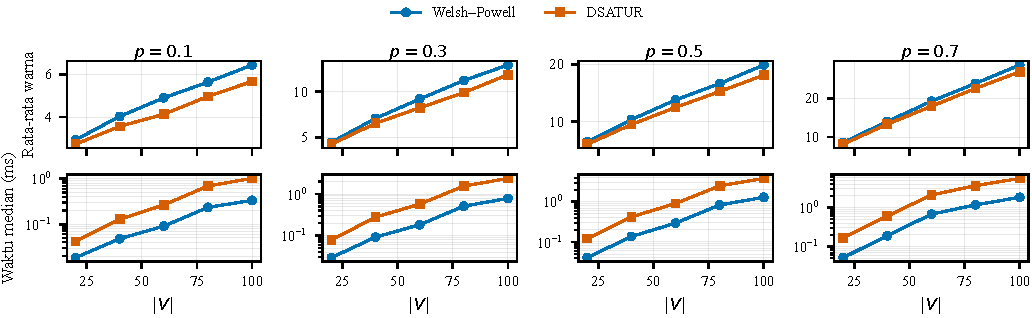
\includegraphics[width=\textwidth]{figures/fig_size_effects.pdf}
\caption{Rata-rata jumlah warna (baris atas) dan waktu eksekusi median berskala
logaritmik (baris bawah) terhadap jumlah mata kuliah, dipisah menurut
probabilitas sisi $p$ pada Eksperimen~A. Selisih jumlah warna melebar seiring
ukuran graf dan menyempit seiring kepadatan, sedangkan DSATUR lebih lambat
pada setiap konfigurasi.}
\label{fig:size}
\end{figure*}

Pola pertumbuhannya sesuai dengan analisis kompleksitas di
Bagian~\ref{sec:algo}. Welsh--Powell tumbuh mendekati linear terhadap $n+m$,
sedangkan DSATUR menunjukkan kemiringan lebih curam karena biaya
$O((n+m)\log n)$ dan biaya tambahan pengelolaan \emph{heap}. Pada $|V|=100$ dan
$p=0.7$, waktu median DSATUR mencapai 5.59 ms dibandingkan 1.83 ms
Welsh--Powell. Angka absolut maupun rasionya bergantung pada mesin uji, bahasa
pemrograman, dan detail implementasi seperti struktur data dan pola alokasi,
sehingga keduanya hanya berlaku untuk implementasi yang diuji di sini; yang
lebih dapat digeneralisasi adalah pola pertumbuhan asimtotiknya.

\subsection{RQ4: Kondisi Keunggulan Masing-Masing}
Gbr.~\ref{fig:size} dan Tabel~\ref{tab:stats} memisahkan hasil menurut
ukuran dan kepadatan. Reduksi rata-rata naik dari 5.23\% pada $|V|=20$ menjadi
10.34\% pada $|V|=60$, lalu sedikit menurun menjadi 8.61\% pada $|V|=100$.
Dengan demikian DSATUR paling menguntungkan pada graf berukuran sedang hingga
besar yang tidak terlalu padat, yaitu kondisi yang paling menyerupai graf
konflik mata kuliah yang sebenarnya.

% generated by src/make_tables.py -- do not edit
\begin{table}[!t]
\centering
\caption{Perbandingan berpasangan jumlah warna. $\Delta k$ adalah rata-rata $k_{\mathrm{DSATUR}}-k_{\mathrm{WP}}$; $r$ adalah korelasi peringkat-biserial; $p$ adalah nilai-$p$ Wilcoxon dua sisi; $p_{\mathrm{Holm}}$ adalah nilai yang disesuaikan dalam keluarga subkelompok.}
\label{tab:stats}
\footnotesize
\setlength{\tabcolsep}{3pt}
\begin{tabular}{@{}lrrrrr@{}}
\toprule
Blok & $\Delta k$ & $R_k$ & $r$ & $p$ & $p_{\mathrm{Holm}}$ \\
\midrule
Semua & -0.794 & 7.17 & -0.946 & $4.2\times10^{-66}$ & -- \\
A, $p=0.1$ & -0.573 & 11.14 & -0.977 & $4.4\times10^{-18}$ & $8.8\times10^{-18}$ \\
A, $p=0.3$ & -0.820 & 8.19 & -0.985 & $2.0\times10^{-18}$ & $6.0\times10^{-18}$ \\
A, $p=0.5$ & -1.153 & 8.04 & -0.938 & $5.4\times10^{-19}$ & $2.2\times10^{-18}$ \\
A, $p=0.7$ & -1.087 & 5.49 & -0.941 & $7.9\times10^{-18}$ & $8.8\times10^{-18}$ \\
B, kecil & +0.000 & 0.00 & +0.000 & 1.000 & 1.000 \\
B, menengah & -0.067 & 0.48 & -1.000 & 0.157 & 0.472 \\
B, besar & -0.033 & 0.11 & -0.200 & 0.655 & 1.000 \\
\bottomrule
\end{tabular}
\end{table}


Sebaliknya, Welsh--Powell tetap kompetitif ketika graf kecil atau sangat padat.
Pada $|V|=20$ dan $p=0.1$, 24 dari 30 instans berakhir seri; pada $p=0.5$ dan
$p=0.7$ dengan ukuran yang sama, Welsh--Powell menang pada tiga dan satu
instans. Karena Welsh--Powell juga sekitar tiga kali lebih cepat, selisih satu
warna pada graf kecil sering tidak sepadan dengan biaya tambahan DSATUR.

\subsection{Eksperimen B: Graf Pendaftaran Terstruktur}
Hasil pada graf yang diturunkan dari simulasi pendaftaran berbeda secara
kualitatif. Dari 90 instans, 83 berakhir seri, DSATUR menang pada 5 instans,
dan Welsh--Powell menang pada 2 instans. Reduksi
rata-rata hanya 0.00\% untuk program kecil, 0.48\% untuk program menengah, dan
0.11\% untuk program besar; tidak satu pun berbeda secara statistik
($p=1.000$, $p=0.157$, dan $p=0.655$; setelah koreksi Holm, $p=1.000$,
$p=0.472$, dan $p=1.000$). Rata-rata jumlah warna kedua algoritma praktis
berimpit pada ketiga skenario.

Temuan ini penting karena justru graf seperti inilah yang menjadi sasaran
penerapan. Graf pendaftaran memiliki struktur komunitas: mata kuliah dalam
jendela semester yang sama cenderung membentuk kelompok padat, sedangkan
antarjendela relatif renggang. Struktur tersebut membuat urutan derajat dan
urutan saturasi konvergen pada keputusan yang sama. Konsekuensinya, klaim umum
bahwa DSATUR "selalu lebih baik" tidak didukung data ini: pada graf
terstruktur, keduanya hampir selalu setara, dan pada graf acak renggang
keunggulan DSATUR nyata tetapi berbayar dengan waktu eksekusi.

\subsection{Verifikasi Optimalitas}
Tabel~\ref{tab:optimality} merangkum celah optimalitas menurut \eqref{eq:gap}
pada 447 dari 450 instans yang dicoba (99.3\%), yaitu 64.8\% dari seluruh
benchmark. Tiga instans mencapai batas simpul $2\times10^{6}$ dan dilaporkan
sebagai tidak terbukti, bukan sebagai optimum; pada ketiganya batas bawah klik
tepat satu di bawah jumlah warna heuristik, sehingga pencarian harus membuktikan
ketiadaan pewarnaan dengan satu warna lebih sedikit. Secara agregat,
Welsh--Powell memakai rata-rata 15.75\% warna lebih banyak daripada optimum,
sedangkan DSATUR 7.06\%. DSATUR mencapai $\chi(G)$ pada 61.3\% instans dan
Welsh--Powell pada 38.7\%.

% generated by src/make_tables.py -- do not edit
\begin{table}[!t]
\centering
\caption{Celah optimalitas menurut \eqref{eq:gap} pada instans yang $\chi(G)$-nya terbukti. Setiap sel berisi $G_{\mathrm{WP}}/G_{\mathrm{DS}}$ dalam persen; tanda -- berarti sel itu di luar cakupan eksak.}
\label{tab:optimality}
\footnotesize
\setlength{\tabcolsep}{3pt}
\begin{tabular}{@{}lcccc@{}}
\toprule
 & $p=0.1$ & $p=0.3$ & $p=0.5$ & $p=0.7$ \\
\midrule
\multicolumn{5}{@{}l}{\emph{Eksperimen A (acak)}} \\
$|V|=20$ & 10.56/1.11 & 9.17/4.17 & 11.37/3.56 & 7.53/1.73 \\
$|V|=40$ & 23.33/7.50 & 20.78/11.67 & 25.19/14.58 & 17.75/12.21 \\
$|V|=60$ & 22.50/3.33 & 30.89/17.14 & 28.09/15.91 & -- \\
$|V|=80$ & 26.33/11.67 & -- & -- & -- \\
\midrule
\multicolumn{5}{@{}l}{\emph{Eksperimen B (pendaftaran)}} \\
kecil & \multicolumn{4}{c}{0.00/0.00} \\
menengah & \multicolumn{4}{c}{0.78/0.25} \\
besar & \multicolumn{4}{c}{0.45/0.47} \\
\midrule
Total & \multicolumn{4}{c}{15.75/7.06} \\
\bottomrule
\end{tabular}
\end{table}


Pola celahnya memperjelas gambaran pada RQ1. Pada graf acak berukuran 20, kedua
heuristik hampir selalu mendekati optimum (celah DSATUR 1.11--4.17\%), sedangkan
pada $|V|=40$ celahnya membesar (DSATUR 7.50--14.58\%, Welsh--Powell
17.75--25.19\%) dan pada $|V|=60$ dengan $p\ge 0.3$ celah DSATUR mencapai
15.91--17.14\%. Pada $|V|=60$ dan $p=0.5$, DSATUR tidak sekali pun mencapai
$\chi(G)$. Pada graf pendaftaran terstruktur, celah keduanya praktis nol
(0.00--0.78\%) dan DSATUR mencapai optimum pada 89.3--100\% instans.
Keunggulan DSATUR karena itu bukan sekadar perbedaan relatif: pada graf acak
berukuran sedang keduanya jauh dari optimum, dan DSATUR hanya lebih dekat.

\subsection{Studi Kasus pada Graf Pendaftaran Nyata}
Pada graf nyata (Eksperimen~C) dengan 156 mata kuliah dan 1.029 sisi
($d=0.085$), Welsh--Powell dan DSATUR sama-sama memakai 13 warna. Klik
berukuran 13 ditemukan, sehingga $\omega(G)\ge 13$; karena pewarnaan sah dengan
13 warna juga ada, $\chi(G)=13$ terbukti dan kedua heuristik optimal pada
instans ini. DSATUR tetap 3.75 kali lebih lambat (1.58 ms berbanding 0.42 ms).

Secara struktural graf nyata berada di antara kedua keluarga sintetis:
koefisien klasternya 0.649, dibandingkan 0.397 pada Eksperimen~A dan 0.776 pada
Eksperimen~B. Posisi ini menjelaskan mengapa hasilnya menyerupai Eksperimen~B
dan bukan Eksperimen~A: pada graf dengan struktur komunitas yang jelas, kedua
urutan pewarnaan konvergen pada keputusan yang sama, dan keduanya dapat
mencapai optimum.

\subsection{Pembahasan}
Secara agregat, jawaban atas RQ1 adalah DSATUR, dengan tiga kualifikasi:
keunggulannya bergantung pada kepadatan (11.14\% pada $p=0.1$ turun menjadi
5.49\% pada $p=0.7$), hilang pada graf pendaftaran terstruktur, dan pada 447
instans terbukti DSATUR memang lebih dekat ke $\chi(G)$ (celah 7.06\%
berbanding 15.75\%) meskipun keduanya sama-sama jauh dari optimum pada graf
acak berukuran 40. Untuk RQ2, jumlah warna naik seiring kepadatan sedangkan
selisihnya menyusut; untuk RQ3, Welsh--Powell konsisten lebih cepat dengan
faktor sekitar tiga dan keduanya berskala polinomial; untuk RQ4, DSATUR unggul
pada graf acak renggang berukuran sedang hingga besar, Welsh--Powell kompetitif
pada graf kecil atau sangat padat, dan keduanya setara pada graf terstruktur.

Bukti eksak menunjukkan bahwa selisih 7.17\% bukan perbedaan seragam antara
``hampir optimal'' dan ``jauh dari optimal''.

Implikasi praktisnya bersyarat: DSATUR layak dipilih ketika jumlah slot adalah
prioritas dan graf renggang serta besar; Welsh--Powell setara dan lebih
sederhana pada graf kecil, padat, atau berstruktur komunitas jelas.

\section{Keterbatasan}
\label{sec:limits}

\emph{Validitas eksternal.} Sebagian telah diperbaiki: satu graf pendaftaran
nyata yang dianonimkan kini diuji dan pola utamanya bertahan. Namun bukti itu
tetap terbatas pada satu institusi, satu potret pendaftaran ujian, dan satu
graf, serta tidak memuat dosen, ruang, atau slot waktu. Pencarian dataset
tambahan tidak menemukan kandidat layak: satu tanpa lisensi, satu berlisensi
CC BY 4.0 tetapi embargo, dan satu hanya memuat jadwal ujian. Generalisasi ke
institusi lain masih memerlukan data konflik dari institusi tersebut.

\emph{Cakupan model.} Model hanya memuat kendala konflik mata kuliah.
Ketersediaan dosen, kapasitas ruang, durasi kuliah yang berbeda, preferensi
waktu, dan batas beban harian tidak dimodelkan. Sisi konflik dosen hanya dapat
dibentuk bila data memuat penugasan dosen; dataset nyata yang dipakai tidak
memuatnya, sehingga sisi tersebut tidak dibentuk dan tidak dilengkapi dengan
informasi yang dikarang.

\emph{Cakupan algoritma.} Yang dievaluasi hanya dua heuristik konstruktif.
Pencarian eksak dipakai sebagai acuan pada instans kecil, bukan sebagai metode
pesaing; metaheuristik dan pemrograman bilangan bulat tidak dibandingkan.

\emph{Optimalitas.} Bilangan kromatik terbukti pada 447 dari 690 instans
(64.8\%). Untuk 243 instans sisanya, terutama $|V|\ge 80$ dan sel padat pada
$|V|=60$, $\chi(G)$ tidak diketahui dan hanya batas
\eqref{eq:gapbounds} yang berlaku. Tidak ada klaim optimalitas umum, dan celah
optimalitas tidak pernah dilaporkan untuk instans yang belum terbukti.

\emph{Pengukuran waktu.} Waktu bergantung pada perangkat keras, sistem operasi,
versi penerjemah, dan beban mesin. Pembekuan snapshot menghilangkan pergeseran
antarrun dalam pemeriksaan klaim, tetapi tidak membuat nilai absolut maupun
rasio dapat dipindahkan ke lingkungan atau implementasi lain; yang dapat
digeneralisasi hanyalah pola pertumbuhan asimtotiknya.

\emph{Inferensi statistik.} Analisis subkelompok bersifat eksploratif dan
dikoreksi Holm, tetapi tetap tidak konfirmatori.

\section{Kesimpulan}
\label{sec:concl}

Penelitian ini membandingkan Welsh--Powell dan DSATUR \emph{greedy} secara
berpasangan pada 690 instans graf sintetis (600 acak dan 90 pendaftaran),
ditambah satu graf pendaftaran nyata yang dianalisis terpisah, dengan 690
perbandingan langsung, 1.380 eksekusi algoritma utama, dan nol konflik.
DSATUR menghasilkan rata-rata 11.10 warna dibandingkan 11.89 (reduksi 7.17\%;
$p=4.2\times10^{-66}$, $r=-0.95$) dan menang pada 390 dari 690 instans, tetapi
sekitar 3.09 kali lebih lambat; keunggulannya menyusut dari 11.14\% pada
$p=0.1$ menjadi 5.49\% pada $p=0.7$ dan hilang pada graf pendaftaran
terstruktur (83 dari 90 seri).

Verifikasi eksak pada 447 instans menempatkan angka itu dalam konteks optimum:
celah rata-rata Welsh--Powell 15.75\% dan DSATUR 7.06\%, dengan DSATUR mencapai
$\chi(G)$ pada 61.3\% instans. Pada graf nyata, $\chi(G)=13$ terbukti dan kedua
heuristik mencapainya. Kesimpulan yang dapat dipertanggungjawabkan karena itu
bersifat bersyarat: DSATUR lebih tepat ketika jumlah slot adalah prioritas dan
graf renggang serta besar, sedangkan Welsh--Powell lebih tepat ketika waktu
komputasi, kesederhanaan, atau ukuran graf kecil menjadi pertimbangan utama.

\bibliographystyle{IEEEtran}
\bibliography{references}

\end{document}
